% ------------------------------------------------------------
% LaTeX Template für die DHBW zum Schnellstart!
% Original: https://github.wdf.sap.corp/vtgermany/LaTeX-Template-DHBW
% ------------------------------------------------------------
% ---- Präambel mit Angaben zum Dokument
\documentclass[
	fontsize=12pt,           % Leitlinien sprechen von Schriftgröße 12.
	paper=A4,
	twoside=false,
	listof=totoc,            % Tabellen- und Abbildungsverzeichnis ins Inhaltsverzeichnis
	bibliography=totoc,      % Literaturverzeichnis ins Inhaltsverzeichnis aufnehmen
	titlepage,               % Titlepage-Umgebung anstatt \maketitle
	headsepline,             % horizontale Linie unter Kolumnentitel
	abstract,              % Überschrift einschalten, Abstract muss in {abstract}-Umgebung stehen
]{scrreprt}                  % Verwendung von KOMA-Report
\usepackage[utf8]{inputenc}  % UTF8 Encoding einschalten
\usepackage[ngerman]{babel}  % Neue deutsche Rechtschreibung
\usepackage[T1]{fontenc}     % Ausgabe von westeuropäischen Zeichen (auch Umlaute)
\usepackage{microtype}       % Trennung von Wörtern wird besser umgesetzt
\usepackage{lmodern}         % Nicht-gerasterte Schriftarten (bei MikTeX erforderlich)
\usepackage{graphicx}        % Einbinden von Grafiken erlauben
\usepackage{wrapfig}         % Grafiken fließend im Text
\usepackage{setspace}        % Zeilenabstand \singlespacing, \onehalfspaceing, \doublespacing
\usepackage[
	%showframe,                % Ränder anzeigen lassen
	left=2.7cm, right=2.5cm,
	top=2.5cm,  bottom=2.5cm,
	includeheadfoot
]{geometry}                      % Seitenlayout einstellen
\usepackage{scrlayer-scrpage}    % Gestaltung von Fuß- und Kopfzeilen
\usepackage{acronym}             % Abkürzungen, Abkürzungsverzeichnis
\usepackage{titletoc}            % Anpassungen am Inhaltsverzeichnis
\contentsmargin{0.75cm}          % Abstand im Inhaltsverzeichnis zw. Punkt und Seitenzahl
\usepackage[                     % Klickbare Links (enth. auch "nameref", "url" Package)
  hidelinks,                     % Blende die "URL Boxen" aus.
  breaklinks=true                % Breche zu lange URLs am Zeilenende um
]{hyperref}
\usepackage[hypcap=true]{caption}% Anker Anpassung für Referenzen
\urlstyle{same}                  % Aktuelle Schrift auch für URLs
% Anpassung von autoref für Gleichungen (ergänzt runde Klammern) und Algorithm.
% Anstatt "Listing" kann auch z.B. "Code-Ausschnitt" verwendet werden. Dies sollte
% jedoch synchron gehalten werden mit \lstlistingname (siehe weiter unten).
\addto\extrasngerman{%
	\def\equationautorefname~#1\null{Gleichung~(#1)\null}
	\def\lstnumberautorefname{Zeile}
	\def\lstlistingautorefname{Listing}
	\def\algorithmautorefname{Algorithmus}
	% Damit einheitlich "Abschnitt 1.2[.3]" verwendet wird und nicht "Unterabschnitt 1.2.3"
	% \def\subsectionautorefname{Abschnitt}
}

% ---- Abstand verkleinern von der Überschrift 
\renewcommand*{\chapterheadstartvskip}{\vspace*{.5\baselineskip}}

% Hierdurch werden Schusterjungen und Hurenkinder vermieden, d.h. einzelne Wörter
% auf der nächsten Seite oder in einer einzigen Zeile.
% LaTeX kann diese dennoch erzeugen, falls das Layout ansonsten nicht umsetzbar ist.
% Diese Werte sind aber gute Startwerte.
\widowpenalty10000
\clubpenalty10000

% ---- Für das Quellenverzeichnis
\usepackage[
	backend = biber,                % Verweis auf biber
	language = auto,
	style = numeric,                % Nummerierung der Quellen mit Zahlen
	sorting = none,                 % none = Sortierung nach der Erscheinung im Dokument
	sortcites = true,               % Sortiert die Quellen innerhalb eines cite-Befehls
	block = space,                  % Extra Leerzeichen zwischen Blocks
	hyperref = true,                % Links sind klickbar auch in der Quelle
	%backref = true,                % Referenz, auf den Text an die zitierte Stelle
	bibencoding = auto,
	giveninits = true,              % Vornamen werden abgekürzt
	doi=false,                      % DOI nicht anzeigen
	isbn=false,                     % ISBN nicht anzeigen
    alldates=short                  % Datum immer als DD.MM.YYYY anzeigen
]{biblatex}
\addbibresource{Inhalt/literatur.bib}
\setcounter{biburlnumpenalty}{3000}     % Umbruchgrenze für Zahlen
\setcounter{biburlucpenalty}{6000}      % Umbruchgrenze für Großbuchstaben
\setcounter{biburllcpenalty}{9000}      % Umbruchgrenze für Kleinbuchstaben
\DeclareNameAlias{default}{family-given}  % Nachname vor dem Vornamen
\AtBeginBibliography{\renewcommand{\multinamedelim}{\addslash\space
}\renewcommand{\finalnamedelim}{\multinamedelim}}  % Schrägstrich zwischen den Autorennamen
\DefineBibliographyStrings{german}{
  urlseen = {Einsichtnahme:},                      % Ändern des Titels von "besucht am"
}
\usepackage[babel,german=quotes]{csquotes}         % Deutsche Anführungszeichen + Zitate


% ---- Für Mathevorlage
\usepackage{amsmath}    % Erweiterung vom Mathe-Satz
\usepackage{amssymb}    % Lädt amsfonts und weitere Symbole
\usepackage{MnSymbol}   % Für Symbole, die in amssymb nicht enthalten sind.


% ---- Für Quellcodevorlage
\usepackage{scrhack}                    % Hack zur Verw. von listings in KOMA-Script
\usepackage{listings}                   % Darstellung von Quellcode
\usepackage{xcolor}                     % Einfache Verwendung von Farben
% -- Eigene Farben für den Quellcode
\definecolor{JavaLila}{rgb}{0.4,0.1,0.4}
\definecolor{JavaGruen}{rgb}{0.3,0.5,0.4}
\definecolor{JavaBlau}{rgb}{0.0,0.0,1.0}
\definecolor{ABAPKeywordsBlue}{HTML}{6000ff}
\definecolor{ABAPCommentGrey}{HTML}{808080}
\definecolor{ABAPStringGreen}{HTML}{4da619}
\definecolor{PyKeywordsBlue}{HTML}{0000AC}
\definecolor{PyCommentGrey}{HTML}{808080}
\definecolor{PyStringGreen}{HTML}{008080}
% -- Farben für ABAP CDS
\definecolor{CDSString}{HTML}{FF8C00}
\definecolor{CDSKeywords}{HTML}{6000ff}
\definecolor{CDSAnnotation}{HTML}{00BFFF}
\definecolor{CDSComment}{HTML}{808080}
\definecolor{CDSFunc}{HTML}{FF0000}

% -- Default Listing-Styles

\lstset{
	% Das Paket "listings" kann kein UTF-8. Deswegen werden hier 
	% die häufigsten Zeichen definiert (ä,ö,ü,...)
	literate=%
		{á}{{\'a}}1 {é}{{\'e}}1 {í}{{\'i}}1 {ó}{{\'o}}1 {ú}{{\'u}}1
		{Á}{{\'A}}1 {É}{{\'E}}1 {Í}{{\'I}}1 {Ó}{{\'O}}1 {Ú}{{\'U}}1
		{à}{{\`a}}1 {è}{{\`e}}1 {ì}{{\`i}}1 {ò}{{\`o}}1 {ù}{{\`u}}1
		{À}{{\`A}}1 {È}{{\'E}}1 {Ì}{{\`I}}1 {Ò}{{\`O}}1 {Ù}{{\`U}}1
		{ä}{{\"a}}1 {ë}{{\"e}}1 {ï}{{\"i}}1 {ö}{{\"o}}1 {ü}{{\"u}}1
		{Ä}{{\"A}}1 {Ë}{{\"E}}1 {Ï}{{\"I}}1 {Ö}{{\"O}}1 {Ü}{{\"U}}1
		{â}{{\^a}}1 {ê}{{\^e}}1 {î}{{\^i}}1 {ô}{{\^o}}1 {û}{{\^u}}1
		{Â}{{\^A}}1 {Ê}{{\^E}}1 {Î}{{\^I}}1 {Ô}{{\^O}}1 {Û}{{\^U}}1
		{œ}{{\oe}}1 {Œ}{{\OE}}1 {æ}{{\ae}}1 {Æ}{{\AE}}1 {ß}{{\ss}}1
		{ű}{{\H{u}}}1 {Ű}{{\H{U}}}1 {ő}{{\H{o}}}1 {Ő}{{\H{O}}}1
		{ç}{{\c c}}1 {Ç}{{\c C}}1 {ø}{{\o}}1 {å}{{\r a}}1 {Å}{{\r A}}1
		{€}{{\euro}}1 {£}{{\pounds}}1 {«}{{\guillemotleft}}1
		{»}{{\guillemotright}}1 {ñ}{{\~n}}1 {Ñ}{{\~N}}1 {¿}{{?`}}1,
	breaklines=true,        % Breche lange Zeilen um 
	breakatwhitespace=true, % Wenn möglich, bei Leerzeichen umbrechen
	% Symbol für Zeilenumbruch einfügen
	prebreak=\raisebox{0ex}[0ex][0ex]{\ensuremath{\rhookswarrow}},
	postbreak=\raisebox{0ex}[0ex][0ex]{\ensuremath{\rcurvearrowse\space}},
	tabsize=4,                                 % Setze die Breite eines Tabs
	basicstyle=\ttfamily\small,                % Grundsätzlicher Schriftstyle
	columns=fixed,                             % Besseres Schriftbild
	numbers=left,                              % Nummerierung der Zeilen
	%frame=single,                             % Umrandung des Codes
	showstringspaces=false,                    % Keine Leerzeichen hervorheben
	keywordstyle=\color{blue},
	ndkeywordstyle=\bfseries\color{darkgray},
	identifierstyle=\color{black},
	commentstyle=\itshape\color{JavaGruen},   % Kommentare in eigener Farbe
	stringstyle=\color{JavaBlau},             % Strings in eigener Farbe,
	captionpos=b,                             % Bild*unter*schrift
	xleftmargin=5.0ex
}

% ---- Eigener JAVA-Style für den Quellcode
\renewcommand{\ttdefault}{pcr}               % Schriftart, welche auch fett beinhaltet
\lstdefinestyle{EigenerJavaStyle}{
	language=Java,                             % Syntax Highlighting für Java
	%frame=single,                             % Umrandung des Codes
	keywordstyle=\bfseries\color{JavaLila},    % Keywords in eigener Farbe und fett
	commentstyle=\itshape\color{JavaGruen},    % Kommentare in eigener Farbe und italic
	stringstyle=\color{JavaBlau}               % Strings in eigener Farbe
}

% ---- Eigener ABAP-Style für den Quellcode
\renewcommand{\ttdefault}{pcr}
\lstdefinestyle{EigenerABAPStyle}{
	language=[R/3 6.10]ABAP,
	morestring=[b]\|,                          % Für Pipe-Strings
	morestring=[b]\`,                          % für Backtick-Strings
	keywordstyle=\bfseries\color{ABAPKeywordsBlue},
	commentstyle=\itshape\color{ABAPCommentGrey},
	stringstyle=\color{ABAPStringGreen},
	tabsize=2,
	morekeywords={
		types,
		@data,
		as,
		lower,
		start,
		selection,
		order,
		by,
		inner,
		join,
		key,
		end,
		cast
	}
}

% ---- Eigener Python-Style für den Quellcode
\renewcommand{\ttdefault}{pcr}
\lstdefinestyle{EigenerPythonStyle}{
	language=Python,
	columns=flexible,
	keywordstyle=\bfseries\color{PyKeywordsBlue},
	commentstyle=\itshape\color{PyCommentGrey},
	stringstyle=\color{PyStringGreen}
}

%----- ABAP-CDS-View language
\lstdefinelanguage{ABAPCDS}{
	sensitive=false,
	%Keywords
	morekeywords={define,
		view,
		as,
		select,
		from,
		inner,
		join,
		on,
		key,
		case,
		when,
		then,
		else,
		end,
		true,
		false,
		cast,
		where,
		and,
		distinct,
		group,
		by,
		having,
		min,
		sum,
		max,
		count,
		avg
	},
	%Methoden
	morekeywords=[2]{
		div,
		currency\_conversion,
		dats\_days\_between,
		concat\_with\_space,
		dats\_add_days,
		dats\_is\_valid,
		dats\_add\_months,
		unit\_conversion,
		division,
		mod,
		abs,
		floor,
		ceil,
		round,
		concat,
		replace,
		substring,
		left,
		right,
		length
	},
	morecomment=[s][\color{CDSAnnotation}]{@}{:},
	morecomment=[l][\itshape\color{CDSComment}]{//},
	morecomment=[s][\itshape\color{CDSComment}]{/*}{*/},
	morestring=[b][\color{CDSString}]',
	keywordstyle=\bfseries\color{CDSKeywords},
	keywordstyle=[2]\color{CDSFunc}
}

  % Weitere Details sind ausgelagert

\usepackage{algorithm}                  % Für Algorithmen-Umgebung (ähnlich wie lstlistings Umgebung)
\usepackage{algpseudocode}              % Für Pseudocode. Füge "[noend]" hinzu, wenn du kein "endif",
                                        % etc. haben willst.

\makeatletter                           % Sorgt dafür, dass man @ in Namen verwenden kann.
                                        % Ansonsten gibt es in der nächsten Zeile einen Compilefehler.
\renewcommand{\ALG@name}{Algorithmus}   % Umbenennen von "Algorithm" im Header der Listings.
\makeatother                            % Zeichen wieder zurücksetzen
\renewcommand{\lstlistingname}{Listing} % Erlaubt das Umbenennen von "Listing" in anderen Titel.

% ---- Tabellen
\usepackage{booktabs}  % Für schönere Tabellen. Enthält neue Befehle wie \midrule
\usepackage{multirow}  % Mehrzeilige Tabellen
\usepackage{siunitx}   % Für SI Einheiten und das Ausrichten Nachkommastellen
\sisetup{locale=DE, range-phrase={~bis~}, output-decimal-marker={,}} % Damit ein Komma und kein Punkt verwendet wird.
\usepackage{xfrac} % Für siunitx Option "fraction-function=\sfrac"

% ---- Für Definitionsboxen in der Einleitung
\usepackage{amsthm}                     % Liefert die Grundlagen für Theoreme
\usepackage[framemethod=tikz]{mdframed} % Boxen für die Umrandung
% ---- Definition für Highlight Boxen

% ---- Grundsätzliche Definition zum Style
\newtheoremstyle{defi}
  {\topsep}         % Abstand oben
  {\topsep}         % Abstand unten
  {\normalfont}     % Schrift des Bodys
  {0pt}             % Einschub der ersten Zeile
  {\bfseries}       % Darstellung von der Schrift in der Überschrift
  {:}               % Trennzeichen zwischen Überschrift und Body
  {.5em}            % Abstand nach dem Trennzeichen zum Body Text
  {\thmname{#3}}    % Name in eckigen Klammern
\theoremstyle{defi}

% ------ Definition zum Strich vor eines Texts
\newmdtheoremenv[
  hidealllines = true,       % Rahmen komplett ausblenden
  leftline = true,           % Linie links einschalten
  innertopmargin = 0pt,      % Abstand oben
  innerbottommargin = 4pt,   % Abstand unten
  innerrightmargin = 0pt,    % Abstand rechts
  linewidth = 3pt,           % Linienbreite
  linecolor = gray!40,       % Linienfarbe
]{defStrich}{Definition}     % Name der des formats "defStrich"

% ------ Definition zum Eck-Kasten um einen Text
\newmdtheoremenv[
  hidealllines = true,
  innertopmargin = 6pt,
  linecolor = gray!40,
  singleextra={              % Eck-Markierungen für die Definition
    \draw[line width=3pt,gray!50,line cap=rect] (O|-P) -- +(1cm,0pt);
    \draw[line width=3pt,gray!50,line cap=rect] (O|-P) -- +(0pt,-1cm);
    \draw[line width=3pt,gray!50,line cap=rect] (O-|P) -- +(-1cm,0pt);
    \draw[line width=3pt,gray!50,line cap=rect] (O-|P) -- +(0pt,1cm);
  }
]{defEckKasten}{Definition}  % Name der des formats "defEckKasten"  % Weitere Details sind ausgelagert

% ---- Für Todo Notes
\usepackage{todonotes}
\setlength {\marginparwidth }{2cm}      % Abstand für Todo Notizen


% ---- Elektronische Version oder Gedruckte Version?
% ---- Unterschied: Die elektronische Version enthält keinen Platzhalter für die Unterschrift
\usepackage{ifthen}
\newboolean{e-Abgabe}
\setboolean{e-Abgabe}{false}    % false=gedruckte Fassung

% ---- Persönlichen Daten:
\newcommand{\titel}{Das Simpsons-Quiz: Finde deinen Zwilling in Springfield!}
\newcommand{\titelheader}{Simpsons-Quiz}
\newcommand{\arbeit}{Programmentwurf}
\newcommand{\studiengang}{Informatik}
\newcommand{\studienjahr}{2015}
\newcommand{\autor}{Dominik Veith}
\newcommand{\autorReverse}{Veith, Dominik}
\newcommand{\verfassungsort}{Karlsruhe}
\newcommand{\matrikelnr}{3352220}
\newcommand{\kurs}{TINF20B2}
\newcommand{\bearbeitungsmonat}{Dezember 2022}
\newcommand{\abgabe}{28. Mai 2023}
\newcommand{\bearbeitungszeitraum}{04.10.2022 - 28.05.2023}
\newcommand{\firmaName}{SAP SE}
\newcommand{\firmaStrasse}{Dietmar-Hopp-Allee 16}
\newcommand{\firmaPlz}{69190 Walldorf, Deutschland}
\newcommand{\betreuerFirma}{B-Vorname B-Nachname}
\newcommand{\betreuerDhbw}{DH-Vorname DH-Nachname}

% ---- Metainformation für das PDF Dokument
\hypersetup{
	pdftitle    = {\titel},
	pdfsubject  = {\arbeit},
	pdfauthor   = {\autor},
	%pdfkeywords = {Keywords angeben},
	pdfcreator  = {LaTeX},
	%pdfproducer = {in der Regel pdfTeX}
}

% ---- Definition der Kopf- und Fußzeilen
\clearpairofpagestyles                          % Löschen von LaTeX Standard
\automark[section]{chapter}                     % Füllen von section und chapter
\renewcommand*{\chaptermarkformat}{}            % Entfernt die Kapitelnummer
\renewcommand*{\sectionmarkformat}{}            % Entfernt die Sectionnummer
% Angaben [für "plain"]{für "scrheadings"}
\ihead[]{\titelheader}                          % Kopfzeile links
\chead[]{}                                      % Kopfzeile mitte
\ohead[]{\rightmark}                            % Kopfzeile rechts
\ifoot[]{}                                      % Fußzeile links
\cfoot*{\sffamily\pagemark}                     % Fußzeile mitte
\ofoot[]{}                                      % Fußzeile rechts
\KOMAoptions{
   headsepline = 0.2pt,                         % Liniendicke Kopfzeile
   footsepline = false                          % Liniendicke Fußzeile
}


% ---- Hilfreiches
\newcommand{\zB}{z.\,B. }   % "z.B." mit kleinem Leeraum dazwischen (ohne wäre nicht korrekt)
\newcommand{\dash}{d.\,h. }

\newcommand{\code}[1]{\texttt{#1}} % Ist einfacher zu schreiben als ständig \texttt und erlaubt
                                   % Änderungen im Nachhinein, wenn man z.B. Inline-Code anders stylen möchte.

% ---- Silbentrennung (falls LaTeX defaults falsch / nicht gewünscht sind)
\hyphenation{HANA}         % anstatt HA-NA
\hyphenation{Graph-Script} % anstatt GraphS-cript

% ---- Beginn des Dokuments
\begin{document}
\setlength{\parindent}{0pt}              % Keine Paragraphen Einrückung.
                                         % Dafür haben wir den Abstand zwischen den Paragraphen.
\setcounter{secnumdepth}{2}              % Nummerierungstiefe fürs Inhaltsverzeichnis
\setcounter{tocdepth}{1}                 % Tiefe des Inhaltsverzeichnisses. Ggf. so anpassen,
                                         % dass das Verzeichnis auf eine Seite passt.
\sffamily                                % Serifenlose Schrift verwenden.

% ---- Vorspann
% ------ Titelseite
\singlespacing
\thispagestyle{empty}
\begin{titlepage}
\enlargethispage{4cm}

\begin{figure}           % Logo vom Ausbildungsbetrieb und der DHBW
	% \vspace*{-5mm} % Sollte dein Titel zu lang werden, kannst du mit diesem "Hack" 
	%                  den Inhalt der Seite nach oben schieben.
	\begin{minipage}{0.49\textwidth}
		\flushleft
		%
\includegraphics[height=2.5cm]{Bilder/Logos/Logo_SAP.pdf} 
	\end{minipage}
	\hfill
	\begin{minipage}{0.49\textwidth}
		\flushright
		
\includegraphics[height=2.5cm]{Bilder/Logos/Logo_DHBW.pdf} 
	\end{minipage}
\end{figure} 
\vspace*{0.1cm}

\begin{center}
	\huge{\textbf{\titel}}\\[1.5cm]
	\Large{\textbf{\arbeit}}\\[0.5cm]
	% \normalsize{im Rahmen der Prüfung zum\\[1ex] \textbf{Bachelor of Science (B.Sc.)}}\\[0.5cm]
	% \Large{des Studienganges \studiengang}\\[1ex]
	% \normalsize{an der Dualen Hochschule Baden-Württemberg Karlsruhe}\\[1cm]
	\normalsize{von}\\[1ex] \Large{\textbf{\autor}} \\[1cm]
	% Hinweis: Manche Dozenten möchten einen Hinweis auf den Sperrvermerk auf der Titelseite.
	% \large{{\color{red}- Sperrvermerk -}}\\[1cm]
\end{center}

\begin{center}
	\vfill
	\begin{tabular}{ll}
		Abgabedatum:                     & \abgabe \\[0.2cm]
		Bearbeitungszeitraum:            & \bearbeitungszeitraum \\[0.2cm]
		Matrikelnummer, Kurs:            & \matrikelnr , \kurs \\[0.2cm]
		% Ausbildungsfirma:                & \firmaName \\
		%                                  & \firmaStrasse \\
		%                                  & \firmaPlz \\[0.2cm]
		% Betreuer der Ausbildungsfirma:   & \betreuerFirma \\[0.2cm]
		% Gutachter der Dualen Hochschule: & \betreuerDhbw \\[2cm]
	\end{tabular} 
\end{center}
\end{titlepage}
  % Titelseite
\newcounter{savepage}
\pagenumbering{Roman}                    % Römische Seitenzahlen
\onehalfspacing

% ------ Erklärung, Sperrvermerk, Abstact
% \chapter*{Eidesstattliche Erklärung}
Ich versichere hiermit, dass ich meine \arbeit{} mit dem Thema:
\begin{quote}
	\textit{\titel}
\end{quote} 
gemäß § 5 der \enquote{Studien- und Prüfungsordnung DHBW Technik} vom 29. September 2017 selbstständig verfasst und keine anderen als die angegebenen Quellen und Hilfsmittel benutzt habe. Die Arbeit wurde bisher keiner anderen Prüfungsbehörde vorgelegt und auch nicht veröffentlicht.

\vspace{0.25cm}

Ich versichere zudem, dass die eingereichte elektronische Fassung mit der gedruckten Fassung übereinstimmt.

\vspace{1cm}

\verfassungsort, den \today \\[0.5cm]
\ifthenelse{\boolean{e-Abgabe}}
	{\underline{Gez. \autor}}
	{\makebox[6cm]{\hrulefill}}\\ 
\autorReverse

% \chapter*{Sperrvermerk}
Die nachfolgende Arbeit enthält vertrauliche Daten der:
\begin{quote}
	\firmaName \\
	\firmaStrasse \\
	\firmaPlz
\end{quote}

\vspace{0.5cm}

Der Inhalt dieser Arbeit darf weder als Ganzes noch in Auszügen Personen außerhalb des Prüfungsprozesses und des Evaluationsverfahrens zugänglich gemacht werden, sofern keine anderslautende Genehmigung vom Dualen Partner vorliegt.

% \renewcommand{\abstractname}{Abstract} % Veränderter Name für das Abstract
\begin{abstract}
\begin{addmargin}[1.5cm]{1.5cm}        % Erhöhte Ränder, für Abstract Look
\thispagestyle{plain}                  % Seitenzahl auf der Abstract Seite

\begin{center}
\small\textit{- English -}             % Angabe der Sprache für das Abstract
\end{center}

\vspace{0.25cm}

This is the starting point of the Abstract. For the final bachelor thesis, there must be an abstract included in your document. So, start now writing it in German and English. The abstract is a short summary with around 200 to 250 words.

\vspace{0.25cm}

Try to include in this abstract the main question of your work, the methods you used or the main results of your work.


\end{addmargin}
\end{abstract}
%\renewcommand{\abstractname}{Abstract} % Veränderter Name für das Abstract
\begin{abstract}
\begin{addmargin}[1.5cm]{1.5cm}        % Erhöhte Ränder, für Abstract Look
\thispagestyle{plain}                  % Seitenzahl auf der Abstract Seite

\begin{center}
\small\textit{- Deutsch -}             % Angabe der Sprache für das Abstract
\end{center}

\vspace{0.25cm}

Dies ist der Beginn des Abstracts. Für die finale Bachelorarbeit musst du ein Abstract in deinem Dokument mit einbauen. So, schreibe es am besten jetzt in Deutsch und Englisch. Das Abstract ist eine kurze Zusammenfassung mit ca. 200 bis 250 Wörtern.

\vspace{0.25cm}

Versuche in das Abstract folgende Punkte aufzunehmen: Fragestellung der Arbeit, methodische Vorgehensweise oder die Hauptergebnisse deiner Arbeit.


\end{addmargin}
\end{abstract}

% ------ Inhaltsverzeichnis
\singlespacing
\tableofcontents

% ------ Verzeichnisse
\renewcommand*{\chapterpagestyle}{plain}
\pagestyle{plain}
% \chapter*{Formelverzeichnis}
\addcontentsline{toc}{chapter}{Formelverzeichnis} % Hinzufügen zum Inhaltsverzeichnis 

% Definition des neuen Befehls für das Einfügen der Abkürzung der Einheit
\newcommand{\acrounit}[1]{
  \acroextra{\makebox[18mm][l]{\si[per-mode=fraction,fraction-function=\sfrac]{#1}}}
}
\begin{acronym}[dmin] % längstes Kürzel wird verw. für den Abstand zw. Kürzel u. Text

	% Alphabetisch selbst sortieren - nicht verwendete Formeln rausnehmen!
	% Allgemein: \acro{KÜRZEL}[ABKÜRZUNG]{\acrounit{SI-EINHEIT}BESCHREIBUNG}

	\acro{A}[\ensuremath{A}]{\acrounit{mm^2}Fläche}	
	\acro{D}[\ensuremath{D}]{\acrounit{mm}Werkstückdurchmesser}	
	\acro{dmin}[\ensuremath{d\textsubscript{min}}]{\acrounit{mm}kleinster Schaftdurchmesser}	
	\acro{L1}[\ensuremath{L\textsubscript{1}}]{\acrounit{mm}Länge des Werkstückes Nr. 1}	
	\acro{Fwinkel}[]{\acrounit{Grad}Freiwinkel}	
	\acro{Kwinkel}[]{\acrounit{Grad}Keilwinkel}

\end{acronym}

\chapter*{Abkürzungsverzeichnis}
\addcontentsline{toc}{chapter}{Abkürzungsverzeichnis} % Hinzufügen zum Inhaltsverzeichnis 

\begin{acronym}[WYSISWG] % längstes Kürzel wird verw. für den Abstand zw. Kürzel u. Text

	% Alphabetisch selbst sortieren - nicht verwendete Kürzel rausnehmen!
	% \acro{AIR}{Adobe Integrated Runtime}
	% \acro{AJAX}{Asynchronous Javascript and XML}
	% \acro{ANSI}{American National Standards Institute}
	% \acro{API}{Application Programming Interface}
	% \acro{AR}{Augmented Reality}
	% \acro{BAPI}{Business Application Programming Interface}
	% \acro{BIOS}{Basic Input Output System}
	% \acro{CDMA}{Code Division Multiple Access}
	% \acro{HTTPS}{Hypertext Transfer Protocol Secure}
	% \acro{ISBN}{Internationale Standardbuchnummer}
	% \acrodefplural{ISBN}[ISBNs]{Internationale Standardbuchnummern}
	% \acro{OLAP}{Online Analytical Processing}
	% \acro{ORDBMS}{Object-Relational DataBase Management System}
	% \acro{SDK}{Software Development Kit}
	% \acro{SEO}{Search Engine Optimization}
	% \acro{SSH}{Secure Shell}
	% \acro{UEFI}{Unified Extensible Firmware Interface}
	% \acro{USB}{Universal Serial Bus}
	% \acro{VLAN}{Virtual Local Area Network}
	% \acro{WYSISWG}{What You See Is What You Get}
	% \acro{XSL}{Extensible Stylesheet Language}
	\acro{JDK}{Java Development Kit}
	\acro{IDE}{Integrated Development Environment}
	\acro{ASCII}{American Standard Code for Information Interchange}

\end{acronym}
\listoffigures                          % Erzeugen des Abbildungsverzeichnisses 
%\listoftables                           % Erzeugen des Tabellenverzeichnisses
\renewcommand{\lstlistlistingname}{Quellcodeverzeichnis}
\lstlistoflistings                      % Erzeugen des Listenverzeichnisses
\setcounter{savepage}{\value{page}}


% ---- Inhalt der Arbeit
\cleardoublepage
\pagenumbering{arabic}                  % Arabische Seitenzahlen für den Hauptteil
\setlength{\parskip}{0.5\baselineskip}  % Abstand zwischen Absätzen
\rmfamily
\renewcommand*{\chapterpagestyle}{scrheadings}
\pagestyle{scrheadings}
\onehalfspacing
\include{Inhalt/05_Inhalt/01_einführung}
\chapter{Clean Architecture}
Dieses Kapitel befasst sich mit der Clean Architecture.
\section{Was ist Clean Architecture?}
% allgemeine Beschreibung der Clean Architecture in eigenen Worten

\section{Analyse der Dependency Rule}
% (1 Klasse, die die Dependency Rule einhält und eine Klasse, die die Dependency Rule verletzt);   jeweils UML der Klasse und Analyse der Abhängigkeiten in beide Richtungen (d.h., von wem hängt die Klasse ab und wer hängt von der Klasse ab) in Bezug auf die Dependency Rule

\subsection{Positiv-Beispiel: Dependency Rule}

\subsection{Negativ-Beispiel: Dependency Rule}

\section{Analyse der Schichten}
% jeweils 1 Klasse zu 2 unterschiedlichen Schichten der Clean-Architecture: jeweils UML der Klasse (ggf. auch zusammenspielenden Klassen), Beschreibung der Aufgabe, Einordnung mit Begründung in die Clean-Architecture

\chapter{SOLID}

\section{Analyse Single-Responsibility-Principle (SRP)}
% jeweils eine Klasse als positives und negatives Beispiel für SRP;  jeweils UML der Klasse und Beschreibung der Aufgabe bzw. der Aufgaben und möglicher Lösungsweg des Negativ-Beispiels (inkl. UML)

\subsection{Positiv-Beispiel}

\subsection{Negativ-Beispiel}

\section{Analyse Open-Closed-Principle (OCP)}
% jeweils eine Klasse als positives und negatives Beispiel für OCP;  jeweils UML der Klasse und Analyse mit Begründung, warum das OCP erfüllt/nicht erfüllt wurde – falls erfüllt: warum hier sinnvoll/welches Problem gab es? Falls nicht erfüllt: wie könnte man es lösen (inkl. UML)?

\subsection{Positiv-Beispiel}

\subsection{Negativ-Beispiel}

\section{Analyse Liskov-Substitution- (LSP), Interface-Segreggation- (ISP), Dependency-Inversion-Principle (DIP)}
% jeweils eine Klasse als positives und negatives Beispiel für entweder LSP oder ISP oder DIP);  jeweils UML der Klasse und Begründung, warum man hier das Prinzip erfüllt/nicht erfüllt wird

\subsection{Positiv-Beispiel}

\subsection{Negativ-Beispiel}
\chapter{Weitere Prinzipien}
General Responsibility Assignment Software Patterns (GRASP) sind eine Sammlung von Prinzipien, welche in der Softwareentwicklung verwendet werden. In diesem Kapitel werden die Prinzipien Geringe Kopplung und Hohe Kohäsion vorgestellt. Außerdem wird das Prinzip Don't Repeat Yourself (DRY) vorgestellt.
\section{Analyse GRASP: Geringe Kopplung}
% jeweils eine bis jetzt noch nicht behandelte Klasse als positives und negatives Beispiel geringer Kopplung; jeweils UML Diagramm mit zusammenspielenden Klassen, Aufgabenbeschreibung und Begründung für die Umsetzung der geringen Kopplung bzw. Beschreibung, wie die Kopplung aufgelöst werden kann
Low Coupling bezeichnet eine geringe Kopplung zwischen Klassen. Eine geringe Kopplung zwischen Klassen bedeutet, dass eine Klasse nur auf wenige andere Klassen angewiesen ist. Eine Klasse, die auf viele andere Klassen angewiesen ist, ist schwieriger zu warten und zu erweitern. Außerdem ist es schwieriger, die Funktionalität einer Klasse zu testen, wenn diese auf viele andere Klassen angewiesen ist. Zusätzlich lässt sie sich einfacher tauschen oder ersetzen. 
\newpage
\subsection{Positiv-Beispiel}
Ein Beispiel, bei dem das Prinzip der Geringen Kopplung umgesetzt wurde ist die Klasse FlandersHome als Beispiel für die verschiedenen Klassen aus dem Package Homes, welche die Wohnungen der Simpsons Figuren repräsentiert. Wie in Abbildung \ref{fig:flandersHome} zu sehen ist, ist die Klasse FlandersHome nur von der Klasse Home abhängig. Zusätzlich implementiert sie notwendige Methoden des HomeFeature Interfaces. Gibt es beispielsweise eine Änderung am Heim von Rektor Skinner, betrifft es diese Klasse nicht.  
\begin{figure}[ht]
    \centering
    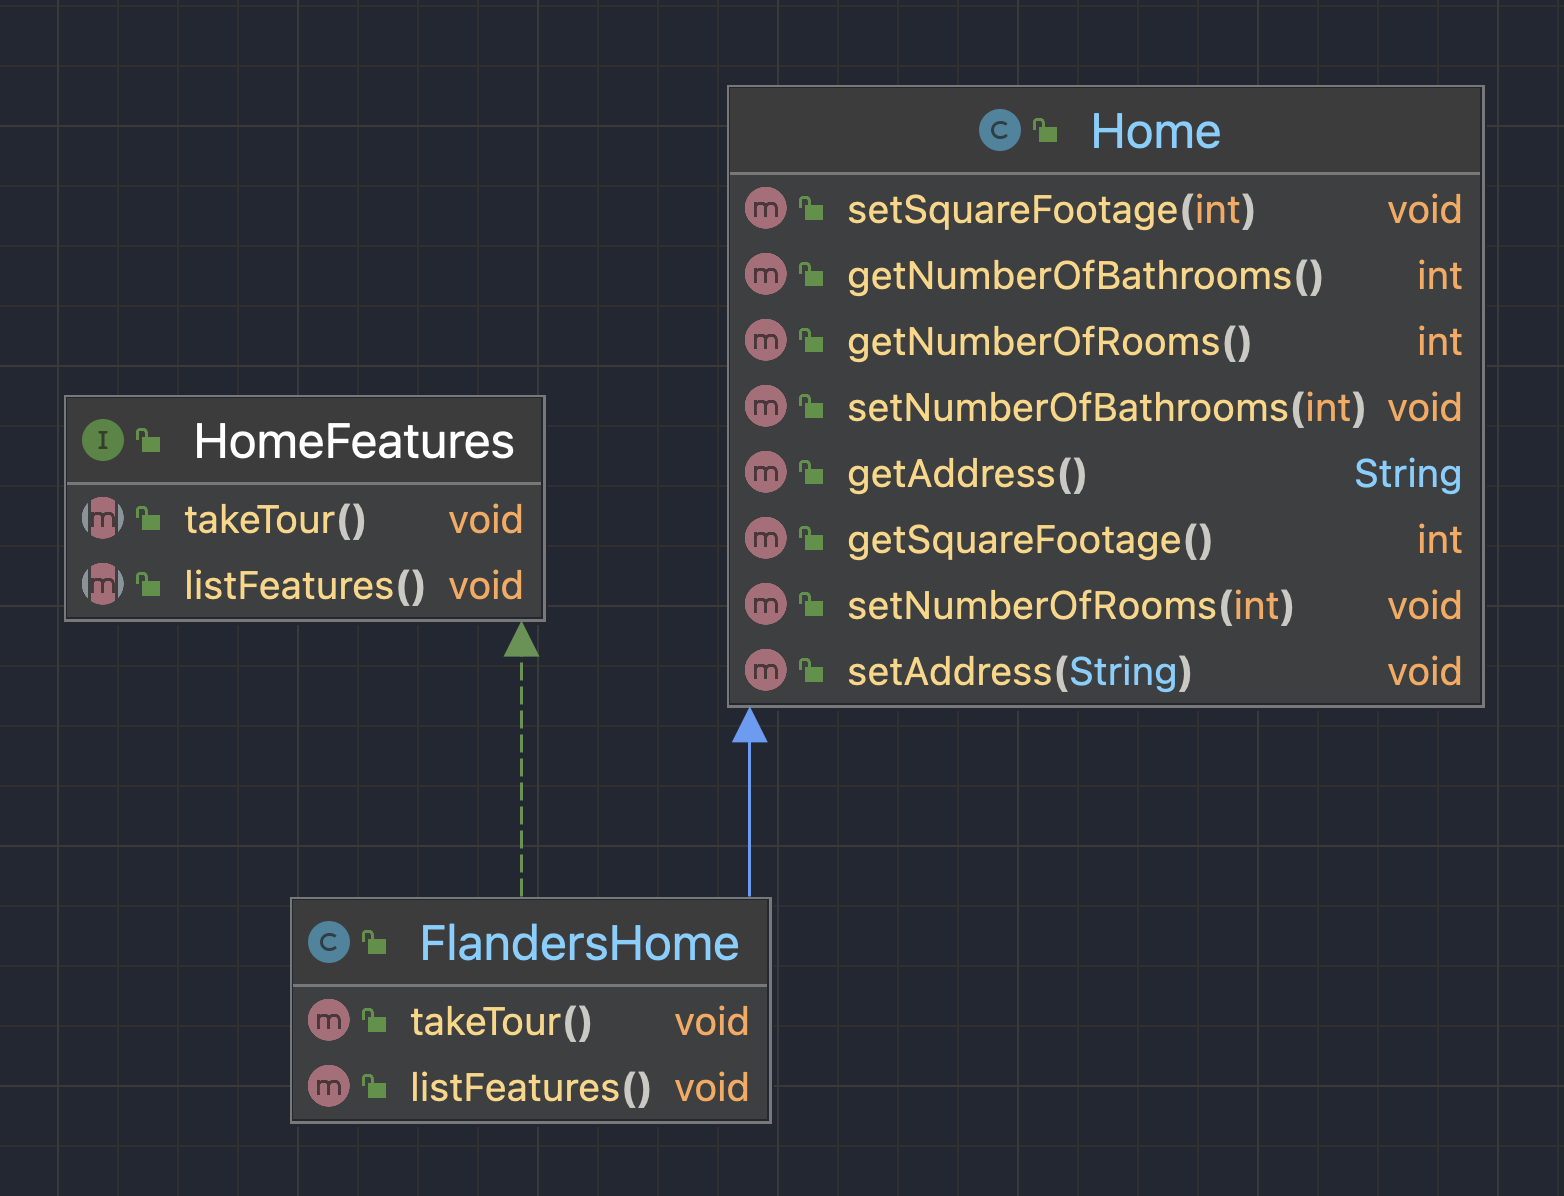
\includegraphics[width=0.3\textwidth]{Bilder/homeI.png}
    \caption{UML Klassendiagramm (FlandersHome) im Zusammenspiel mit Interface}
    \label{fig:flandersHome}
\end{figure}

\subsection{Negativ-Beispiel}
Führt man das zuvor genannte Beispiel eine Ebene nach oben, wird allerdings deutlich, dass die Klasse QuestionManager von jeder Klasse, welche eine der Simpsons Figuren repräsentiert, abhängig ist und somit eine hohe Kopplung aufweist. Abbildung \ref{fig:hoheK} zeigt die Klasse QuestionManager im Zusammenspiel mit den Klassen aus dem Package der Charaktere. 
\begin{figure}[ht]
    \centering
    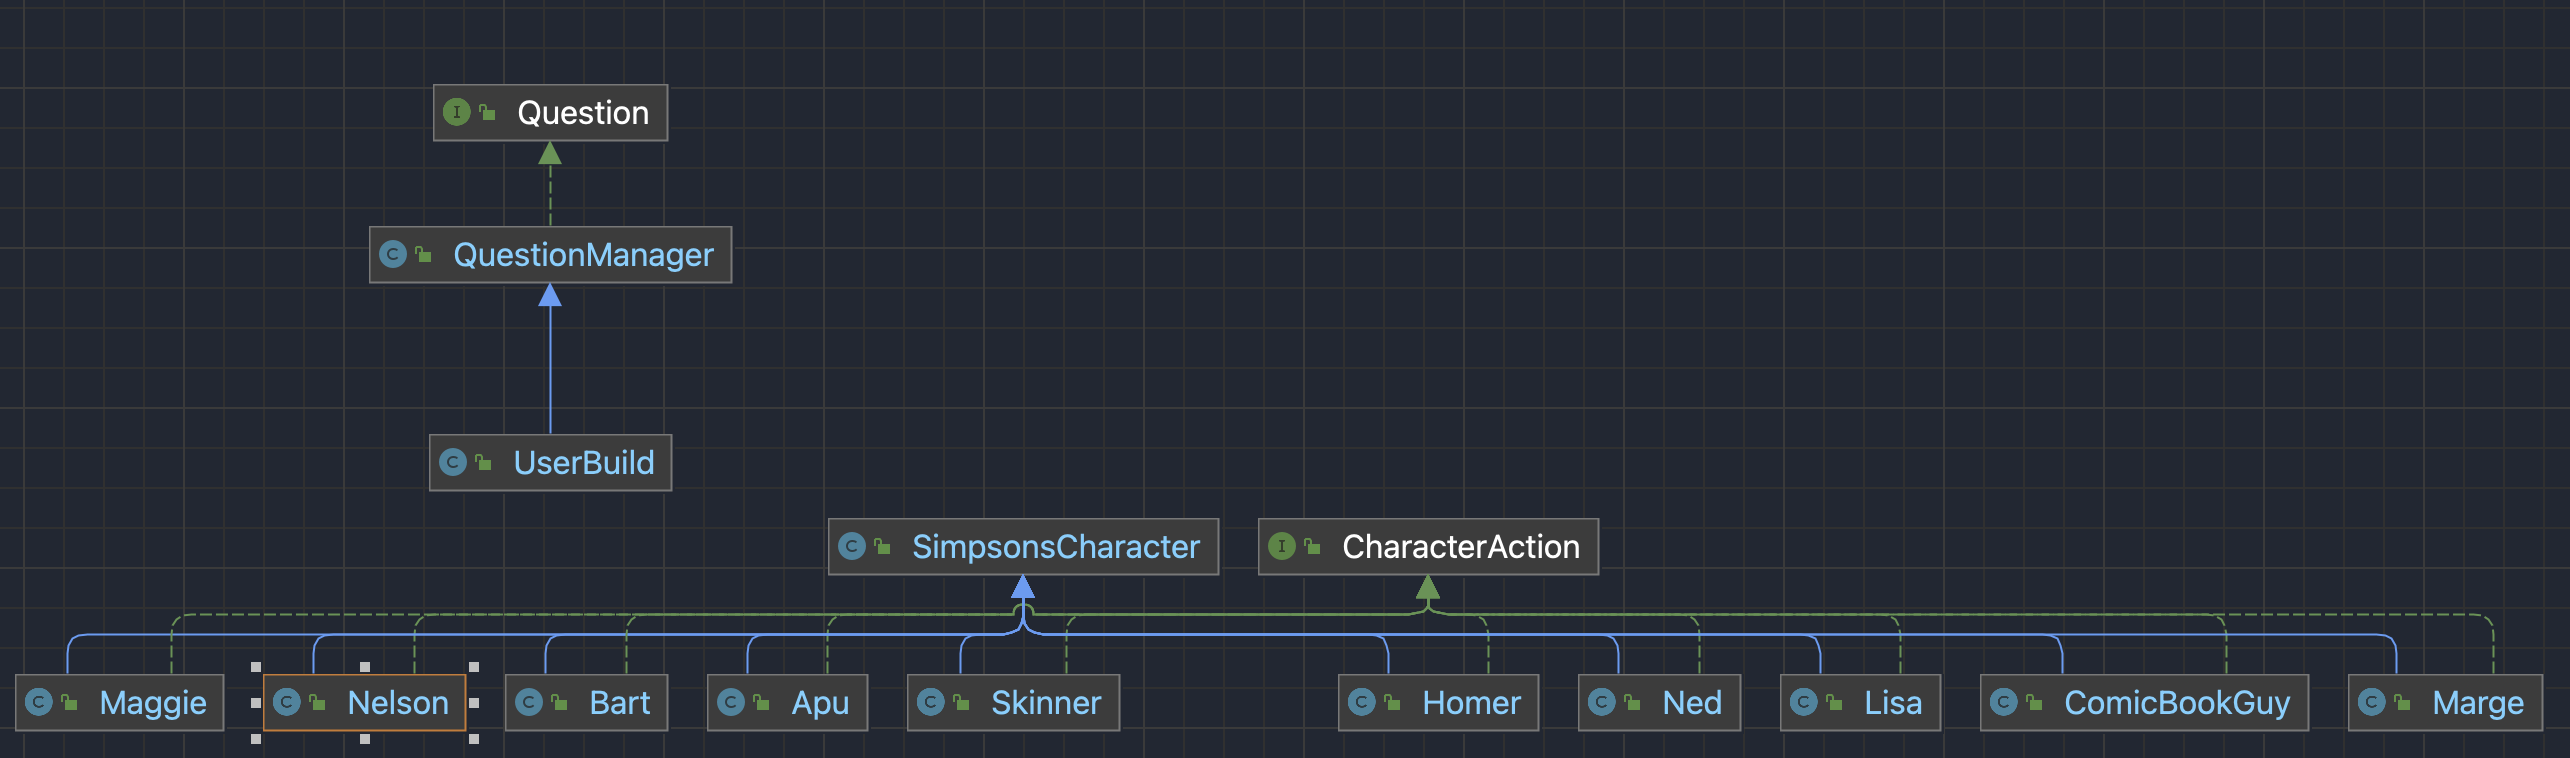
\includegraphics[width=0.8\textwidth]{Bilder/hoheK.png}
    \caption{UML Klassendiagramm (QuestionManager) in Abhängigkeit der Charaktere}
    \label{fig:hoheK}
\end{figure}

\section{Analyse GRASP: Hohe Kohäsion}
% eine Klasse als positives Beispiel hoher Kohäsion; UML Diagramm und Begründung, warum die Kohäsion hoch ist
Hohe Kohäsion ist wichtig, da Objekte so organisiert werden sollten, dass die Methoden und Attribute zusammengehören und eine klar definierte Aufgabe erfüllen. Zusätzlich erhöht es wesentlich die Überschaubarkeit und des Codes. Abbildung \ref{fig:highK} zeigt die Klassen der einzelnen Figuren im Zusammenhang mit ihren Arbeitsstätten und Wohnorte.
\begin{figure}[ht]
    \centering
    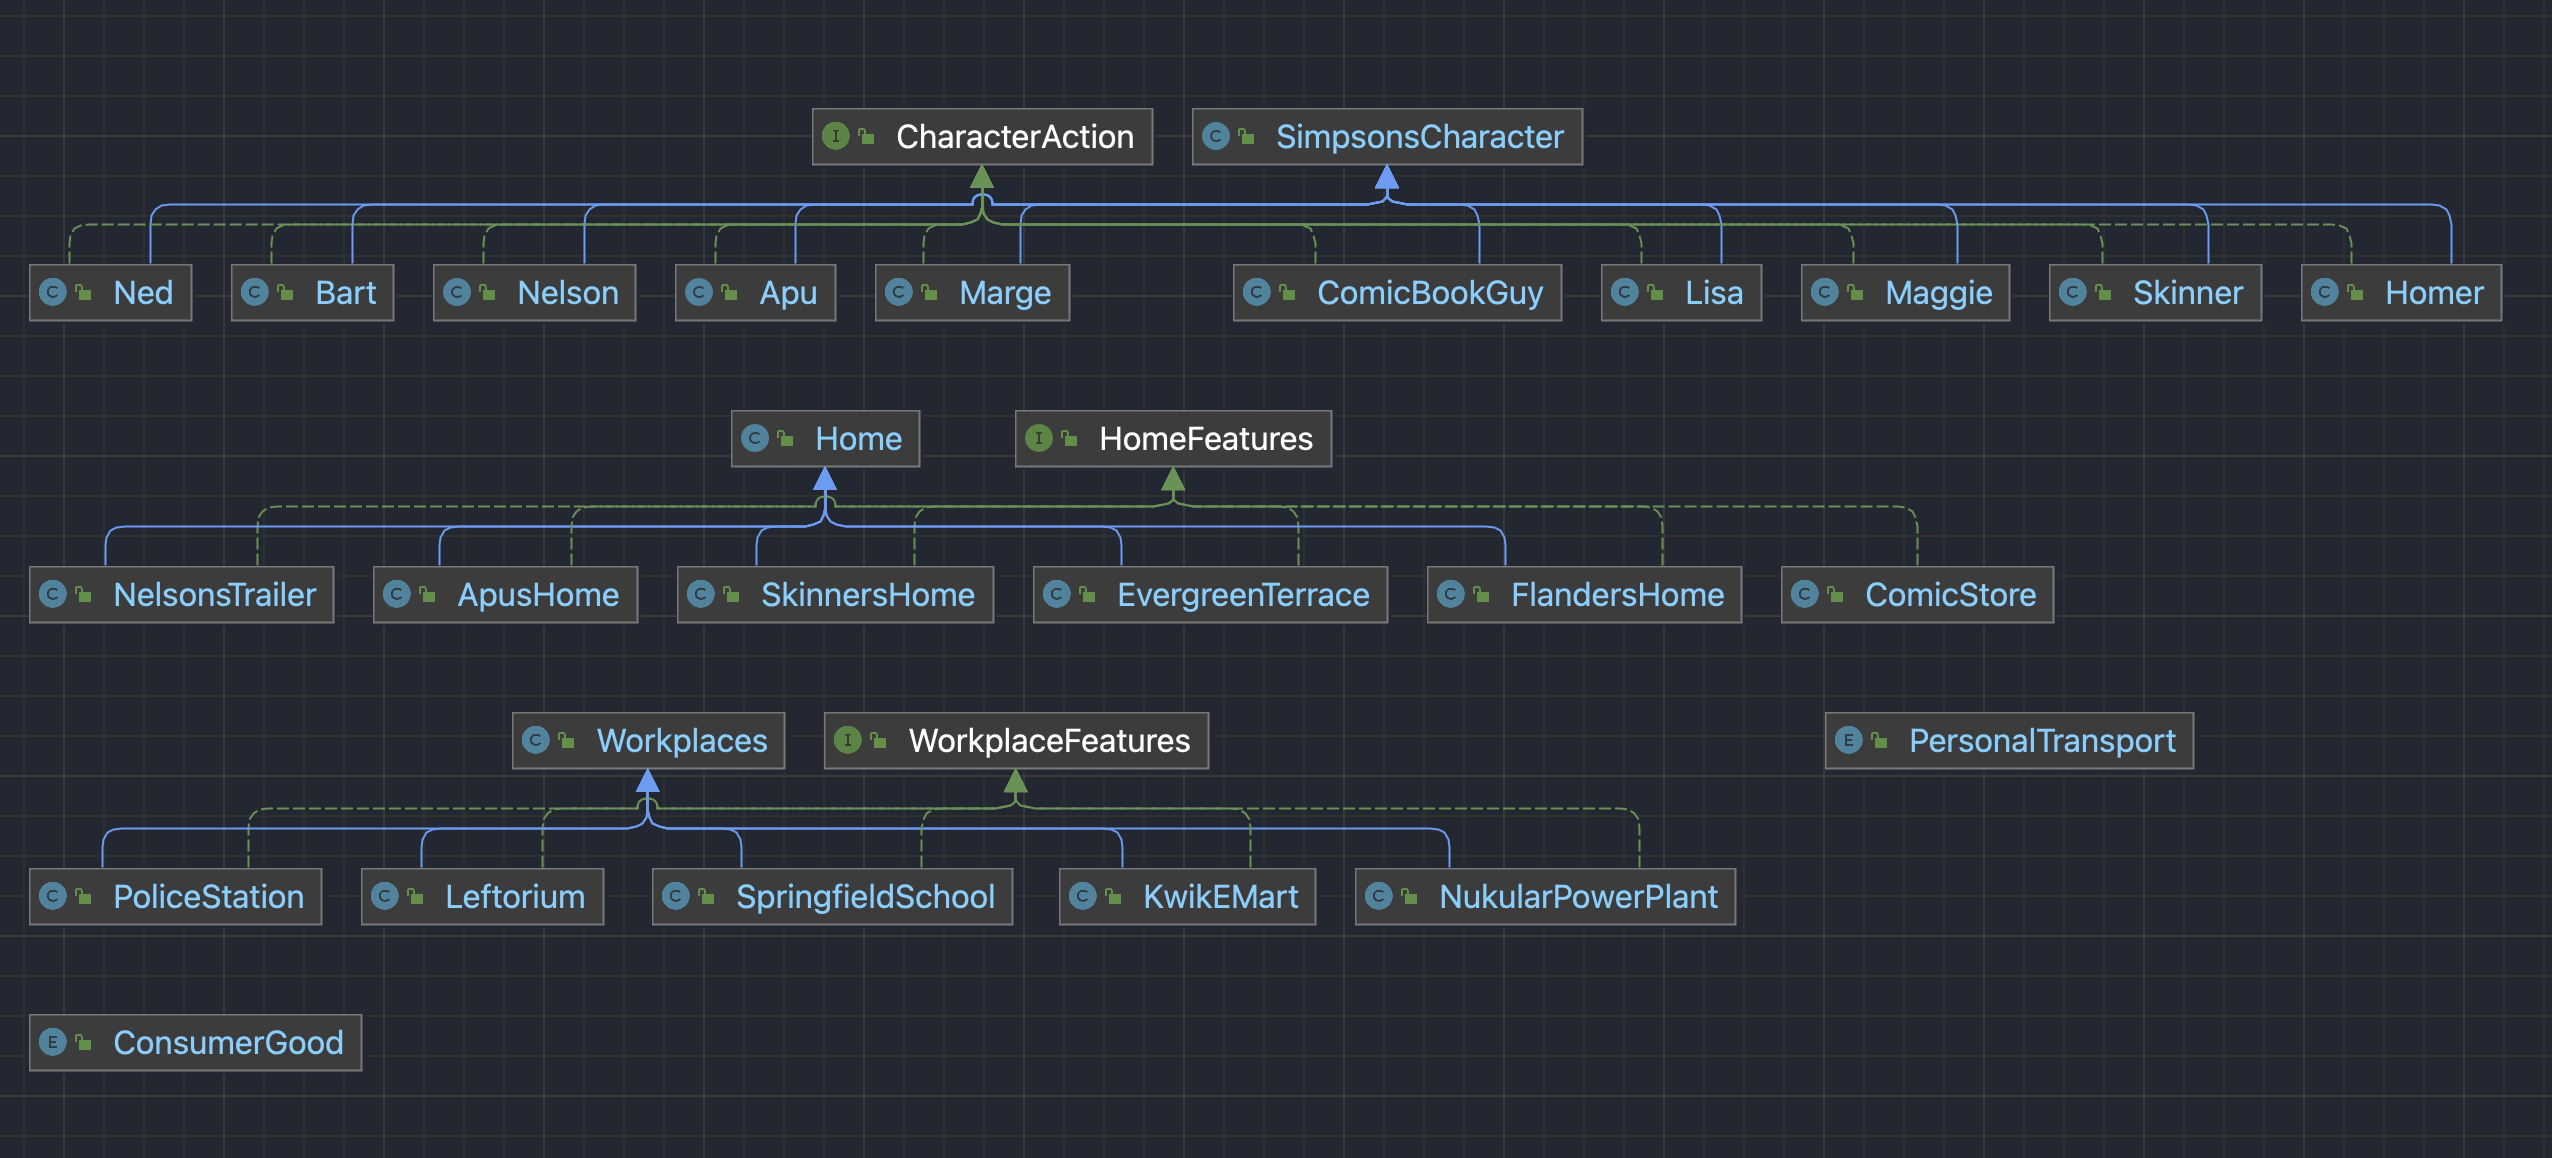
\includegraphics[width=0.8\textwidth]{Bilder/highK.png}
    \caption{UML Klassendiagramm (Charaktere im Zusammenspiel mit Arbeitsstätte und Zuhause)}
    \label{fig:highK}
\end{figure}
\newpage

\section{Don't Repeat Yourself (DRY)}
% ein Commit angeben, bei dem duplizierter Code/duplizierte Logik aufgelöst wurde; Code-Beispiele (vorher/nachher); begründen und Auswirkung beschreiben
DRY ist ein Akronym für Don't Repeat Yourself und ein weiteres Prinzip der Softwareentwicklung. Es bedeutet, dass jede Funktionalität oder Information in einem Programm nur einmal definiert werden sollte um Redundanzen zu vermeiden. So kann beispielsweise Code ausgelagert werden um ihn wiederverwenden zu können ohne ihn zu duplizieren. Außerdem wird die Wartbarkeit des Codes erhöht, da Änderungen nur an einer Stelle vorgenommen werden müssen. So wurde beispielsweise, wie in Listing \ref{code:DRY} zu sehen ist, der Code für die Ausgabe der Charakter Bilder in die SimpsonsCharacter Klasse ausgelagert und kann so direkt von den jeweiligen Klassen aufgerufen werden.
\lstinputlisting[
    label={code:DRY},  % Label; genutzt für Referenzen auf dieses Code-Beispiel
	caption={DRY Prinzip bei Ausgabe der Charakter Bilder},  % Caption; genutzt für Referenzen auf dieses Code-Beispiel
	captionpos=b,               % Position, für die Caption:  t(op) oder b(ottom)
	style=EigenerJavaStyle,     % Eigener Style der vor dem Dokument festgelegt wurde
	firstline=1,                % Zeilennummer im Dokument welche als erste angezeigt wird
	lastline=10     
]{Quellcode/Picture.java}
\chapter{Unit Tests}
% Beschreibung der Tests
Unit Tests haben die Aufgabe einzelne Einheiten von Code auf Funktionalität zu überprüfen. Dabei kann eine Einheit eine einzelne Methode, eine Klasse oder ein Modul sein. Zweck ist die Sicherstellung dass jede Einheit der Software wie erwartet funktioniert und dass Änderungen an einer Einheit keine unerwarteten Auswirkungen auf andere Teile der Software haben. Darüber hinaus helfen Unit-Tests auch dabei, die Qualität und Zuverlässigkeit der Software zu verbessern, da sie sicherstellen, dass jeder Teil des Codes wie erwartet funktioniert und dass Fehler vermieden werden. Unit-Tests tragen somit dazu bei, dass die Software insgesamt stabiler und robuster wird.
\section{10 Unit Tests}
%Nennung von 10 Unit-Tests und Beschreibung, was getestet wird
\begin{enumerate}
    \item UserBuildTest.testPerformActionBasedOnAnswers() Testet ob für jeden Simpsons Charakter eine Aktion bereitgestellt wird.
    \item ApuTest.testIntroduce() Testet ob die Methode introduce() den richtigen String zurückgibt. Die selben Tests wurden für die Simpsons Charaktere Bart, Homer, Marge, Lisa, Maggie, ComicBookGuy, Ned, Skinner und Nelson durchgeführt.
    \item SimpsonsCharacterTest.testFavoriteFood() Testet ob abhängig vom Charakter der Simpsons das spezifische Lieblingsessen zurückgegeben wird.
    \item SimpsonsCharacterTest.testPersonalTransport() Testet ob abhängig vom Charakter der Simpsons das spezifische Transportmittel zurückgegeben wird.
    \item ConsumerGoodsTest.testToString() Testet ob abhängig vom jeweiligen Enum der richtige String zum Lieblingsessen zurückgegeben wird.
    \item PersonalTransportTest.testDisplayName() Testet ob abhängig vom jeweiligen Enum der richtige String zum Transportmittel zurückgegeben wird.
    \item WorkplacesTest.testGettersAndSetters() Testet ob die Getter und Setter der Klasse Workplaces funktionieren.
\end{enumerate}

\section{ATRIP: Automatic}
%Begründung/Erläuterung, wie ‘Automatic’ realisiert wurde
Test sollten nach Möglichkeit automatisiert ablaufen. Des Weiteren sollten auch die Ergebnisse eines Tests auf ihren positiven oder negativen Ausgang geprüft werden. In diesem Projekt wird dies mit dem Surfire Plugin von Maven realisiert, welches, wie in Abbildung \ref{fig:surefire} zu sehen, alle Tests auf einmal abruft und angibt, ob ein Test fehlgeschlagen ist oder nicht. Abgerufen wird dieser Test mit dem Befehl 'mvn test' im Verzeichnis des Projekts über das Terminal.
\begin{figure}[ht]
    \centering
    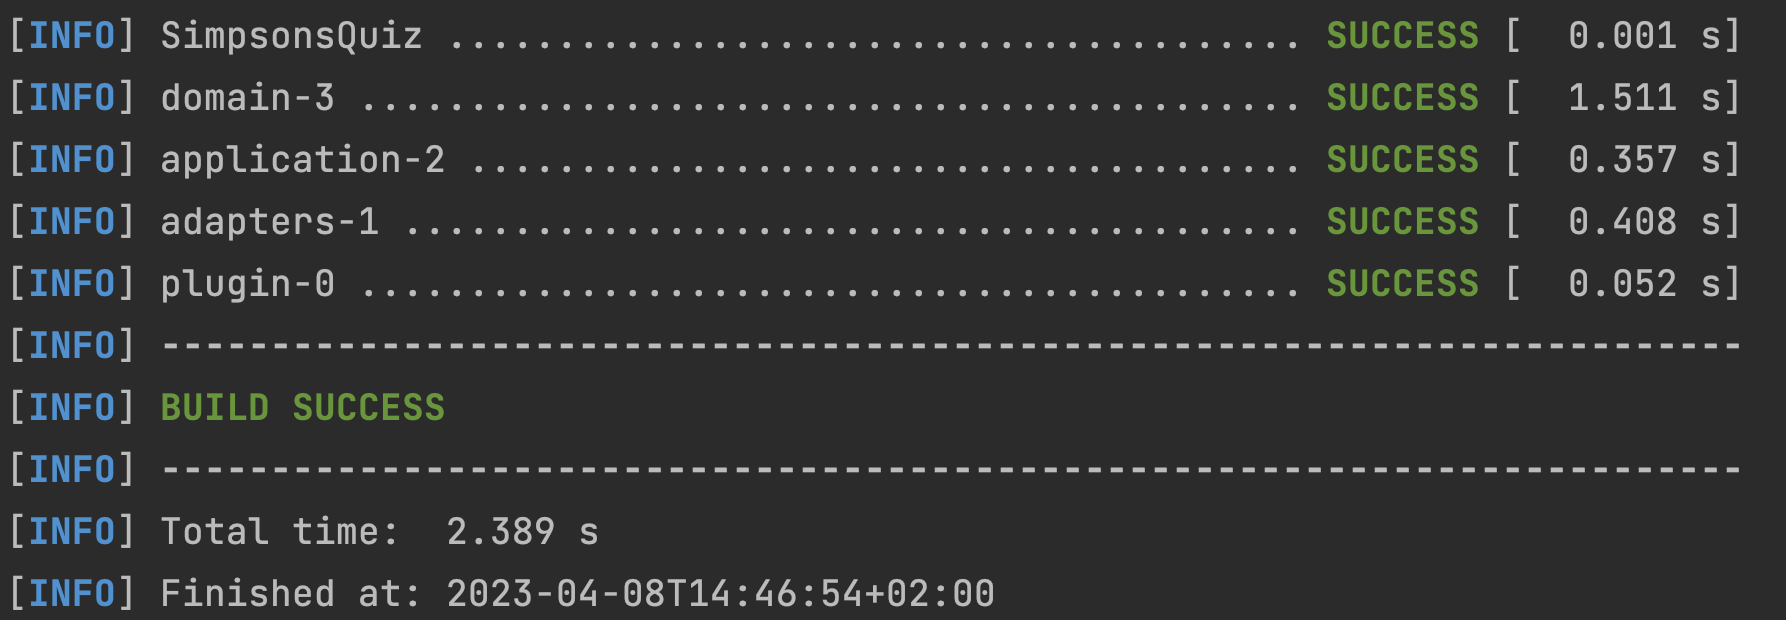
\includegraphics[width=0.8\textwidth]{Bilder/tests.png}
    \caption{Maven Surfire Plugin}
    \label{fig:surefire}
\end{figure}
\newpage

\section{ATRIP: Thorough}
% jeweils 1 positives und negatives Beispiel zu ‘Thorough’; jeweils Code-Beispiel, Analyse und Begründung, was gründlich/nicht gründlich ist
Thorough bezieht sich auf die Gründlichkeit eines Tests, insbesondere auf die vollständige Prüfung des gesamten Codes um sicherzustellen, dass alle Aspekte der Funktionalität geprüft und alle Szenarien abgedeckt wurden. In diesem Projekt wurde dies durch die Erstellung von Unit Tests für jeden einzelnen Simpsons Charakter sichergestellt, wie in listing \ref{code:apuTest} zu sehen ist. Die Tests prüfen, ob die Methode introduce() den richtigen String zurückgibt. Die selben Tests wurden für die Simpsons Charaktere Bart, Homer, Marge, Lisa, Maggie, ComicBookGuy, Ned, Skinner und Nelson durchgeführt.

\lstinputlisting[
	label=code:apuTest,    % Label; genutzt für Referenzen auf dieses Code-Beispiel
	caption=Unit Test der Klasse Apu,
	captionpos=b,               % Position, an der die Caption angezeigt wird t(op) oder b(ottom)
	style=EigenerJavaStyle,     % Eigener Style der vor dem Dokument festgelegt wurde
	firstline=1,                % Zeilennummer im Dokument welche als erste angezeigt wird
	lastline=12                 % Letzte Zeile welche ins LaTeX Dokument übernommen wird
]{Quellcode/apu.java}
Negativ gilt an dieser Stelle hervorzuheben, dass nicht alle Methoden der jeweiligen Klassen getestet werden. Nur wenn alle Methoden vollständig durch Unit Tests abgedeckt sind, gilt das Prinzip erfüllt.  
\section{ATRIP: Professional}
% jeweils 1 positives und negatives Beispiel zu ‘Professional’; jeweils Code-Beispiel, Analyse und Begründung, was professionell/nicht professionell ist
Da Tests den selben Qualitätsstandards wie Produktivcode unterliegen, sollte auch hierbei darauf geachtet werden, dass die Tests mit der notwendigen Professionalität erstellt werden. Dies bedeutet, dass die Tests gut lesbar und wartbar sind. Außerdem sollten sie so geschrieben werden, dass sie leicht zu verstehen sind und dass sie sich leicht erweitern lassen. Ein positives Beispiel ist die der Test des User Builds in listing \ref{code:userBuildTest}. Dieser Test prüft, ob für jeden Simpsons Charakter eine Aktion bereitgestellt wird. Dies wird durch die Methode testPerformActionBasedOnAnswers() realisiert. Dabei spielt es keine Rolle wie viele Charakter momentan vorhanden sind, oder ob noch welche hinzugefügt werden. 
\lstinputlisting[
    label=code:userBuildTest,    % Label; genutzt für Referenzen auf dieses Code-Beispiel
    caption=Unit Test der Klasse UserBuild,
    captionpos=b,               % Position, an der die Caption angezeigt wird t(op) oder b(ottom)
    style=EigenerJavaStyle,     % Eigender Style der vor dem Dokument festgelegt wurde
    firstline=1,                % Zeilennummer im Dokument welche als erste angezeigt wird
    lastline=9                 % Letzte Zeile welche ins LaTeX Dokument übernommen wird
]{Quellcode/goodtest.java} 
\newpage

Unnötige Tests wie beispielsweise der Test von Getter und Setter Methoden sind hingegen nicht professionell. Dies ist in listing \ref{code:badtest} zu sehen. Dieser Test prüft, ob die Getter und Setter der Klasse Workplaces funktionieren. Dies ist unnötig, da man keine Tests nur des Testens wegen schreiben sollte.
\lstinputlisting[
    label=code:badtest,    % Label; genutzt für Referenzen auf dieses Code-Beispiel
    caption=Unit Test der Klasse Workplaces,
    captionpos=b,               % Position, an der die Caption angezeigt wird t(op) oder b(ottom)
    style=EigenerJavaStyle,     % Eigender Style der vor dem Dokument festgelegt wurde
    firstline=1,                % Zeilennummer im Dokument welche als erste angezeigt wird
    lastline=23                 % Letzte Zeile welche ins LaTeX Dokument übernommen wird
]{Quellcode/badtest.java}
\newpage

\section{Code Coverage}
% Code Coverage im Projekt analysieren und begründen
Code Coverage ist ein Maß dafür, wie viel Prozent des Quellcodes einer Software durch Tests abgedeckt werden. Eine Code Coverage von 100\% würde bedeuten, dass jeder Teil des Codes durch Tests abgedeckt wurde, während eine  niedrigere Code Coverage darauf hinweist, dass einige Teile des Codes nicht durch Tests überprüft wurden. In diesem Projekt wurde die Code Coverage mit dem JaCoCo Plugin von Maven ermittelt. Dieses Plugin ist in Abbildung \ref{fig:jacoco} zu sehen. Die Code Coverage beträgt 24\% der Klassen und 17\% der Methoden, womit also noch Bedarf an Optimierung besteht.
\begin{figure}[ht]
    \centering
    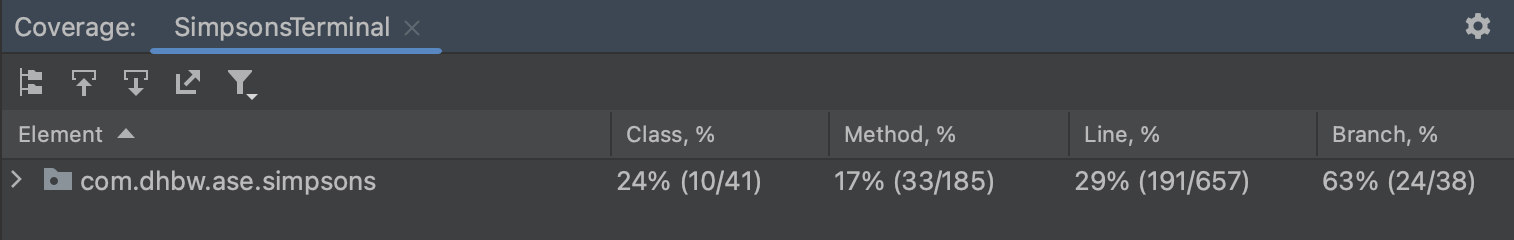
\includegraphics[width=0.8\textwidth]{Bilder/coverage.png}
    \caption{Maven JaCoCo Plugin}
    \label{fig:jacoco}
\end{figure}
\newpage

\section{Fakes und Mocks}
% Analyse und Begründung des Einsatzes von 2 Fake/Mock-Objekten; zusätzlich jeweils UML Diagramm der Klasse
Mocks sind im Kontext von Unit-Tests Platzhalter-Objekte, die das Verhalten von Abhängigkeiten simulieren, die für den Test nicht verfügbar sind oder unerwünschte Nebenwirkungen haben könnten. Sie helfen, Tests schneller auszuführen, indem sie die Interaktionen der zu testenden Komponente mit ihren Abhängigkeiten imitieren. Mocks können auch zur Überprüfung von Interaktionen verwendet werden, indem sie aufgezeichnete Methodenaufrufe und Parameter speichern und anschließend überprüfen, ob sie den erwarteten Werten entsprechen. In diesem Projekt wird, wie in listing \ref{code:mock} zu sehen, der Unit Test QuestionManagerTest als Mock Klasse verwendet um die Eingabe durch einen Nutzer zu simulieren. 
\lstinputlisting[
    label=code:mock,    % Label; genutzt für Referenzen auf dieses Code-Beispiel
    caption=Mock Klasse für den Question Manager,
    captionpos=b,               % Position, an der die Caption angezeigt wird t(op) oder b(ottom)
    style=EigenerJavaStyle,     % Eigender Style der vor dem Dokument festgelegt wurde
    firstline=1,                % Zeilennummer im Dokument welche als erste angezeigt wird
    lastline=33                 % Letzte Zeile welche ins LaTeX Dokument übernommen wird
]{Quellcode/mock.java}

Die Mock-Klasse enthält eine Test-Methode testAskQuestions (), die eine Instanz von QuestionManager erstellt und die askQuestions() - Methode dieser Instanz testet. Zunächst wird eine zufällige Benutzereingabe erstellt, indem eine StringBuilder-Instanz mit der Größe der charToName-Map der QuestionManager-Klasse initialisiert wird. Die Schleife durchläuft dann jede Zeichenposition und fügt zufällig 'y' für Ja oder 'n' für Nein hinzu, um die Benutzereingabe zu simulieren. Anschließend wird eine InputStream-Instanz erstellt, um die generierte Benutzereingabe zu setzen. Dann wird die askQuestions () -Methode aufgerufen, um die Antwort des Frage-Managers zu erhalten. Schließlich wird geprüft, ob das Ergebnis ein gültiges Zeichen enthält, das in der Liste der erwarteten Zeichen "validChars" enthalten ist.
\chapter{Domain Driven Design}
Domain Driven Design ist ein Ansatz der Software Entwicklung, bei dem die Domäne und deren Logik im Mittelpunkt steht. Dabei hilft DDD der Komplexität von Software vorzubeugen, indem es den Fokus auf das Verständnis der Domäne legt. \cite{ddd.2003}
\section{Ubiquitous Language}
% 4 Beispiele für die Ubiquitous Language; jeweils Bezeichnung, Bedeutung und kurze Begründung, warum es zur Ubiquitous Language gehört
Ubiquitous Language ist ein zentrales Konzept im Domain-Driven Design und bezieht sich auf eine gemeinsame, konsistente Sprache, die von allen Beteiligten im Projekt verwendet wird, um die Domäne und ihre Anforderungen zu beschreiben. Diese einheitliche Sprache soll Kommunikationsprobleme zwischen Entwicklern, Fachexperten, Stakeholdern und anderen Teammitgliedern vermeiden und ein gemeinsames Verständnis der Domäne fördern. In der Praxis bedeutet dies, dass die Begriffe, die in der Geschäftsdomäne verwendet werden, konsistent in den Diskussionen, Dokumentationen und im Code selbst verwendet werden sollten. Ubiquitous Language wird im gesamten Entwicklungsprozess eingesetzt, von der Anforderungsanalyse über das Design bis hin zur Implementierung.
Im Folgenden wird die Ubiquitous Language des Simpsons Quiz Projekts vorgestellt.
\begin{itemize}
    \item Charakter: Ein Charakter ist eine Person der Simpsons Serie. Dabei ist es egal ob es sich um einen Hauptcharakter oder einen Nebencharakter handelt.
    \item Picture: Ein Picture ist ein Bild, welches einem Charakter der Serie zugeordnet ist.
    \item Workplace: Ein Workplace ist ein Arbeitsplatz, welcher einem Charakter der Serie zugeordnet ist.
    \item Home: Ein Home ist ein Wohnort, welcher einem Charakter der Serie zugeordnet ist.
    \item LuxuryFood: Ein LuxuryFood ist das Lieblingsessen, welches einem Charakter der Serie zugeordnet ist.
    \item Transport: Ein Transport ist das präferierte  Transportmittel, welches einem Charakter der Serie zugeordnet ist.
\end{itemize}
Die Begriffe zählen zur Ubiquitous Language, da sie essentiell für das Verständnis des Simpsons Quiz sind und die Hauptmerkmale des Aufbaus der jeweiligen Figur im Rahmen des Quiz darstellen. Dabei werden sie bei der Implementierung als Gruppierung der einzelnen Attribute verwendet.
\section{Entities}
% UML, Beschreibung und Begründung des Einsatzes einer Entity; falls keine Entity vorhanden: ausführliche Begründung, warum es keines geben kann/hier nicht sinnvoll ist
Entitäten repräsentieren Objekte, die innerhalb einer Geschäftsdomäne eine eindeutige Identität besitzen. Im Gegensatz zu Value Objects, die nur durch ihre Attribute definiert sind, haben Entitäten eine Identität, die unabhängig von ihren Eigenschaften ist. Das bedeutet, dass selbst wenn sich der Zustand einer Entität im Laufe der Zeit ändert, ihre Identität konstant bleibt. Beispiele für Entitäten können Kunden, Produkte, Bestellungen oder Mitarbeiter sein. In all diesen Fällen ist die Identität des Objekts entscheidend, um es von anderen Objekten desselben Typs unterscheiden zu können. Im Simpsons Quiz stellen Charakter, Workplace, Home, LuxuryFood und Transport Entitäten dar.
\newpage

\section{Value Objects}
% UML, Beschreibung und Begründung des Einsatzes eines Value Objects; falls kein Value Object vorhanden: ausführliche Begründung, warum es keines geben kann/hier nicht sinnvoll ist
Value Objects sind ein wichtiger Bestandteil von Domain-Driven Design (DDD) und repräsentieren Objekte, die keine eigene Identität haben und ausschließlich durch ihre Eigenschaften oder Attribute definiert sind. Im Gegensatz zu Entitäten, die eine eindeutige Identität besitzen und deren Zustand sich im Laufe der Zeit ändern kann, sind Value
Objects unveränderlich und können bei Bedarf einfach ersetzt werden. Im Simpsons Quiz stellen die einzelne Charaktere des Spiels Value Objects dar. Sie sind anhand ihrer Attribute wie Arbeitsplätze, Vorlieben oder Zitaten einzigartig und können nur durch einen anderen Charakter ersetzt, aber nicht verändert werden.
\begin{figure}[ht]
    \centering
    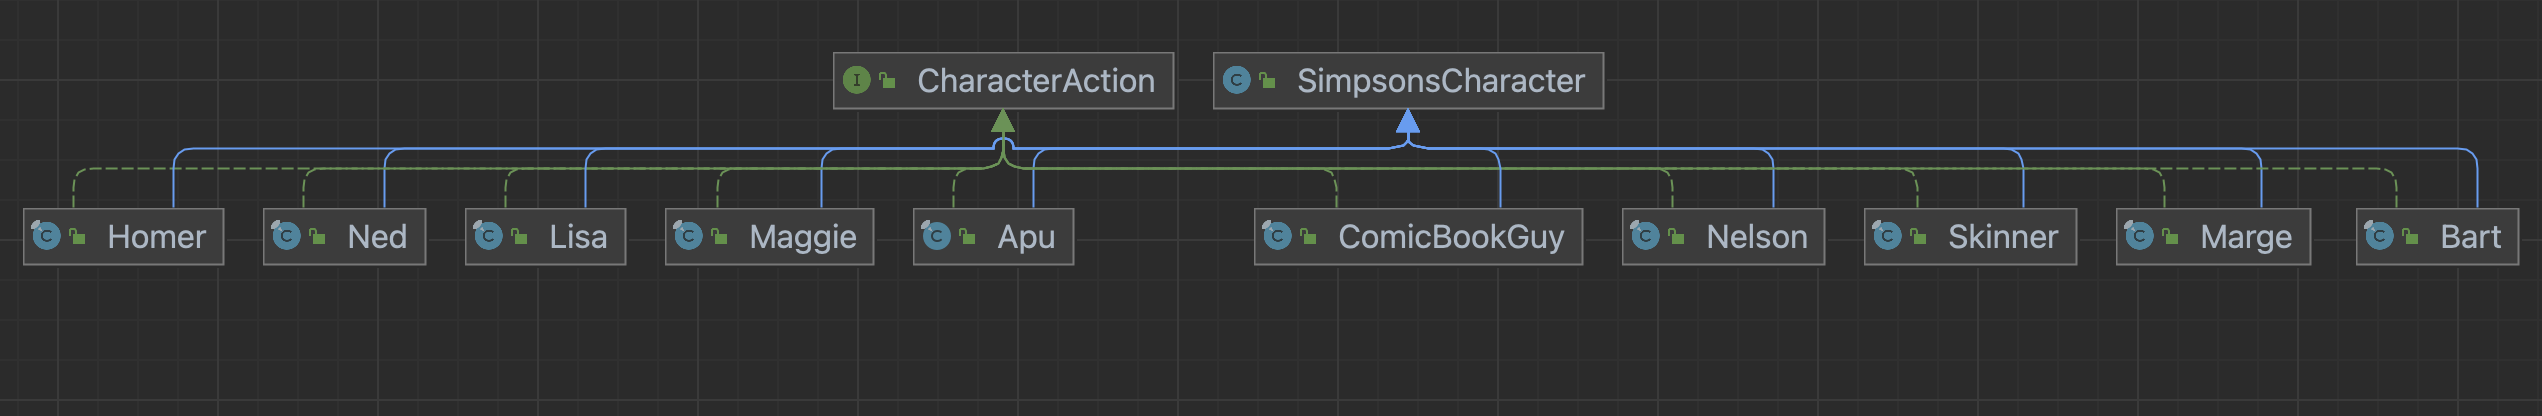
\includegraphics[width=0.9\textwidth]{Bilder/charakter.png}
    \caption{UML Diagramm für Value Objects}
    \label{fig:ValueObject}
\end{figure}

\section{Repositories}

Repositories vermitteln zwischen der Domäne und dem Modell und stellen Methoden bereit um Aggregates aus dem Persistenzspeicher zu lesen oder zu speichern. Im Simpsons Quiz werden keine Repositories verwendet, da die Abfrage des Aggregates bereits alle Informationen liefert und somit eine weitere Abstraktionsebene überflüssig macht. 

\section{Aggregates}
% UML, Beschreibung und Begründung des Einsatzes eines Aggregates; falls kein Aggregate vorhanden: ausführliche Begründung, warum es keines geben kann/hier nicht sinnvoll ist
Aggregates beziehen sich auf eine Gruppe von zusammenhängenden Entitäten und Value Objects, die eine konsistente Geschäftseinheit bilden. Dabei ist genau geregelt, welche Entitäten und Value Objects zu einem Aggregate gehören und welche nicht, um die Abhängigkeiten abzubilden. \newline
Im Simpsons Quiz gibt es das Aggregate UserBuild, welches aus den Entitäten Charakter, Workplace, Home, LuxuryFood und Transport besteht und mit den Value Objects die Spiel Figur zusammenstellt.

\chapter{Refactoring}

\section{Code Smells}
%[jeweils 1 Code-Beispiel zu 2 Code Smells aus der Vorlesung; jeweils Code-Beispiel und einen möglichen Lösungsweg bzw. den genommen Lösungsweg beschreiben (inkl. (Pseudo-)Code)
Code Smells sind Anzeichen oder Muster in der Software, die auf mögliche Probleme oder schlechte Praktiken im Code hindeuten. Sie sind nicht unbedingt Fehler oder Bugs, können jedoch die Wartbarkeit, Lesbarkeit und Qualität des Codes beeinträchtigen. In diesem Kapitel werden zwei Code Smells im Projekt vorgestellt behoben.
\subsection{Code Smell: Duplicated Code}
Das Vorhandensein von ähnlichem oder identischem Code an mehreren Stellen im Projekt kann auf schlechte Modularisierung oder mangelnde Wiederverwendbarkeit hindeuten. Jeder Simpsons Charakter hat neben seinen Attributen und Methoden, welche sein Zuhause oder Transportmittel beschreiben, auch eine Methode welche nachdem der Charakter ausgewählt wurde, ein entsprechendes Bild über das Terminal ausgibt. Dieser Code ist in allen Charakterklassen vorhanden und wird in jeder Klasse aufgerufen. Dieser Code ist also mehrfach vorhanden und kann durch Auslagern in eine Superklasse gelöst werden. Wie in listing \ref{code:Picture} zu sehen wurde die Methode in die Superklasse SimpsonsCharacter ausgelagert und in den jeweiligen Subklassen nur noch aufgerufen.
\lstinputlisting[
    label=code:Picture,    % Label; genutzt für Referenzen auf dieses Code-Beispiel
    caption=Auslagern der Methode printPicture() in die Superklasse SimpsonsCharacter, % Caption; genutzt für Referenzen auf dieses Code-Beispiel
    captionpos=b,               % Position, an der die Caption angezeigt wird t(op) oder b(ottom)
    style=EigenerJavaStyle,     % Eigender Style der vor dem Dokument festgelegt wurde
    firstline=1,                % Zeilennummer im Dokument welche als erste angezeigt wird
    lastline=10                 % Letzte Zeile welche ins LaTeX Dokument übernommen wird
]{Quellcode/printpicture.java} 


\subsection{Code Smell: Large Class}
Eine Large Class ist eine Klasse, die zu viele Methoden oder eine große Anzahl von Codezeilen hat. Dies kann ein Anzeichen dafür sein, dass die Klasse zu viele Verantwortlichkeiten trägt. Eine große Klasse kann es schwierig machen, den Code zu verstehen, zu warten und zu erweitern. Um dieses Problem zu lösen, sollte die Klasse in kleinere, fokussierte Klassen aufgeteilt werden, die jeweils eine einzige Verantwortung haben. Im Simpsons Quiz gibt es für jeden Charakter bereits eine separate Klasse. Allerdings war bis vor dem Refactoring die Bilder der Charakter ebenfalls mit in der Klasse gespeichert. Das Auslagern in extra Klassen sorgt für eine deutliche Reduktion der Code Zeilen der Charakter Klassen. Im Folgenden Commit sind die Änderungen zu sehen:
\url{https://github.com/Crixos86/AdvancedSE_DHBW/commit/2f4d1b47780bfbeddbe100c476d0e97a3478f384}
\lstinputlisting[
    label=code:picline,    % Label; genutzt für Referenzen auf dieses Code-Beispiel
    caption=Lösung der large class, % Caption; genutzt für Referenzen auf dieses Code-Beispiel
    captionpos=b,               % Position, an der die Caption angezeigt wird t(op) oder b(ottom)
    style=EigenerJavaStyle,     % Eigender Style der vor dem Dokument festgelegt wurde
    firstline=1,                % Zeilennummer im Dokument welche als erste angezeigt wird
    lastline=4                 % Letzte Zeile welche ins LaTeX Dokument übernommen wird
]{Quellcode/picline.java}
\newpage
\section{2 Refactorings}
% 2 unterschiedliche Refactorings aus der Vorlesung anwenden, begründen, sowie UML vorher/nachher liefern; jeweils auf die Commits verweisen
Refactorings sind strukturierte Änderungen am Code, die darauf abzielen, die interne Struktur und Qualität des Codes zu verbessern, ohne das äußere Verhalten oder die Funktionalität der Software zu ändern. Das Hauptziel von Refactoring ist es, den Code lesbarer, wartbarer und besser verständlich zu machen, was die Produktivität der
Entwickler erhöht und die Wahrscheinlichkeit von Fehlern oder Bugs reduziert.
\subsection{Switch Statements}
Im Simpsons Quiz wird je nach Antworten des Spielers ein anderer Charakter der Serie ausgewählt. Dies wurde initial durch ein Switch Statement realisiert was aber nicht sehr gut wartbar ist und auch in Teilen gegen das Open Closed Principle verstößt. Der Code wurde, wie in listing \ref{code:Switch}zu sehen, entsprechend angepasst.
\lstinputlisting[
    label=code:Switch,    % Label; genutzt für Referenzen auf dieses Code-Beispiel
    caption=Refactoring des Switch Statements, % Caption; genutzt für Referenzen auf dieses Code-Beispiel
    captionpos=b,               % Position, an der die Caption angezeigt wird t(op) oder b(ottom)
    style=EigenerJavaStyle,     % Eigender Style der vor dem Dokument festgelegt wurde
    firstline=1,                % Zeilennummer im Dokument welche als erste angezeigt wird
    lastline=16                 % Letzte Zeile welche ins LaTeX Dokument übernommen wird
]{Quellcode/userbuild.java}

Die Verwendung der Runnable Interfaces und einer Map mit Lambdas bieten gegenüber dem Switch Statement einige Vorteile:
\begin{itemize}
    \item Lesbarkeit: Die Verwendung einer Map und Lambdas bietet eine klarere und leichter verständliche Struktur, da sie die Logik zur Ausführung der Aktionen auf einer höheren Abstraktionsebene kapselt.
    \item Erweiterungen: Es ist einfacher, der Map neue Aktionen hinzuzufügen oder vorhandene Aktionen zu ändern, ohne den gesamten Code umzuschreiben. Im Gegensatz dazu erfordert ein Switch-Statement oft eine umfangreichere Änderung des Codes, um neue Fälle hinzuzufügen oder bestehende zu ändern.
    \item Open/Closed Principle: Durch die Verwendung einer Map und Lambdas folgt der Code eher dem Open/Closed Principle, das besagt, dass Software-Einheiten (Klassen, Module, Funktionen usw.) für Erweiterungen offen, aber für Modifikationen geschlossen sein sollten. Hier kann die Implementierung leicht erweitert werden, ohne dass der bestehende Code geändert werden muss.
    \item Effizienz: Da die Map auf Hash-basierten Schlüsseln arbeitet, ist der Zugriff auf die zugehörige Aktion in der Regel schneller als ein Switch-Statement, insbesondere wenn es eine große Anzahl von Fällen gibt.
    \item Flexibilität: Das Runnable-Interface ermöglicht es, Aktionen sowohl synchron als auch asynchron auszuführen. Wenn beispielsweise eine Aktion in einem neuen Thread ausgeführt wird, kann ein Runnable-Objekt an den Thread-Konstruktor übergeben werden.
\end{itemize}
\newpage
\subsection{Polymorphismus}
Polymorphismus ist ein grundlegendes Konzept der objektorientierten Programmierung, das es ermöglicht, verschiedene Objekte durch eine gemeinsame Schnittstelle oder Basisklasse zu behandeln. Polymorphismus kann als Refactoring-Technik verwendet werden, um den Code sauberer, modularer und leichter wartbar zu gestalten. Mit Einführung der SimpsonsCharacter Klasse wurden gemeinsame Eigenschaften und Methoden der Charaktere ausgelagert. Im folgenden Commit ist das Refactoring zu sehen: \url{https://github.com/Crixos86/AdvancedSE_DHBW/commit/7a1e0367ca782b108682dd7c3f19ae087445ccfa} \newline
Folgende Vorteile wurden durch die Einführung der Superklasse erreicht:
\begin{itemize}
    \item Bessere Abstraktion: Polymorphismus ermöglicht es, eine gemeinsame Schnittstelle oder Basisklasse für unterschiedliche Verhaltensweisen oder Implementierungen zu definieren. Dies führt zu einer klareren Abstraktion und kapselt die unterschiedlichen Implementierungen besser.
    \item Erhöhte Wiederverwendbarkeit: Durch die Verwendung von Polymorphismus kann Code, der auf der gemeinsamen Schnittstelle oder Basisklasse basiert, wiederverwendet werden. Dies reduziert die Code-Redundanz und verbessert die Modularität.
    \item Einfachere Erweiterbarkeit: Mit Polymorphismus können neue Verhaltensweisen oder Implementierungen hinzufügt werden, indem neue Klassen erstellt werden, die die gemeinsame Schnittstelle oder Basisklasse erweitern. Dies verbessert die Erweiterbarkeit des Codes und erleichtert das Hinzufügen neuer Funktionen.
\end{itemize}
\chapter{Entwurfsmuster}
% 2 unterschiedliche Entwurfsmuster aus der Vorlesung (oder nach Absprache auch andere) jeweils sinnvoll einsetzen, begründen und UML-Diagramm


% ---- Literaturverzeichnis
\cleardoublepage
\renewcommand*{\chapterpagestyle}{plain}
\pagestyle{plain}
\pagenumbering{Roman}                   % Römische Seitenzahlen
\setcounter{page}{\numexpr\value{savepage}+1}
\printbibliography[title=Literaturverzeichnis]

% ---- Anhang
\appendix
%\clearpage
%\pagenumbering{Roman}  % römische Seitenzahlen für Anhang

\newpage
\end{document}
